\section{Data and Data Collection Methodology}

\subsection{Data Source}

The empirical sample covers Chess.com Titled Tuesday tournaments from February 2022 through April 2026. February 2022 is used as the lower bound because Titled Tuesday itself changed around that period: the prize structure expanded and the event moved into the two-tournament weekly format. Special prizes for women and streamers were also introduced, adding additional participation and ranking incentives. Restricting the pre-period to February 2022 onward avoids mixing the September 2025 reform with an earlier institutional regime.

Table~\ref{tab:titled-tuesday-prizes} reports the weekly prize schedule used as institutional context for the empirical design. The tournament is not only a high-skill repeated game environment; it is also a cash-prize competition with rewards concentrated at the top of the final standings and separate prizes for the top woman and three streamers \citep{chesscom_titled_tuesday}. This matters for interpretation because the same rule change that altered the time control also operated inside a tournament where late-round rank pressure and expected prize returns can affect participation, completion, and risk-taking incentives.

\begin{table}[H]
\centering
\caption{Weekly Titled Tuesday Prize Pool}
\label{tab:titled-tuesday-prizes}
\begin{tabular}{lr}
\toprule
Place or category & Prize \\
\midrule
1st & \$1,000 \\
2nd & \$750 \\
3rd & \$350 \\
4th & \$250 \\
5th & \$150 \\
6th & \$100 \\
Top woman & \$100 \\
Top streamer (x3) & \$100 each \\
\midrule
Total weekly prize pool & \$3,000 \\
\bottomrule
\end{tabular}
\end{table}

The main treatment date is September 2, 2025, the first Titled Tuesday under the new 5+0 no-increment format. In the regression data the post-treatment indicator is denoted \texttt{format\_5\_0}. It equals one for games played after the reform and zero for the old 3+1 period. The pre-period includes the two weekly time slots, while the post-period includes only the remaining main slot. Because the reform bundles time-control and scheduling changes, the analysis separates conditional game-performance outcomes from participation and completion outcomes wherever possible.

\subsection{Tournament and Game Metadata Scraping}

The main data source is a manually compiled player-game dataset built from Chess.com Titled Tuesday tournament pages and associated game links. Chess.com exposes useful information through its public API, but the API is organized primarily around player-month archives rather than tournament-level datasets. This is inconvenient for Titled Tuesday because the research design requires the tournament, round, pairing, standings, and game metadata for each event. The collection process therefore started from Chess.com tournament pages, especially pages under the Titled Tuesday event structure, and scraped round pairings, player names, opponents, colors of pieces, ratings, titles, results, and final leaderboard information. Thus, for each game played in the tournament, we have two observations in the final dataset: one for the player with the white pieces and one for the player with the black pieces.

The move data were collected through a separate pipeline using Chess.com's Published Data API. After the tournament scrape identified game links and player usernames, the script queried each relevant player's monthly public game archive and PGN endpoint, then retained only PGNs whose game URL matched a Titled Tuesday game in the metadata \citep{chesscom_pubapi,chesscom_pgn_api}. This produced the raw move sequences used later for Stockfish evaluation without relying on the Chess.com analysis interface. The PGNs used in this project contain move text, standard game headers, and clock annotations where Chess.com records them. These annotations are parsed into remaining time before the move, remaining time after the move, and time spent on the move, allowing the thesis to study both board-state mechanisms and direct clock-state mechanisms.

\begin{table}[H]
\centering
\caption{Example of the PGN Structure Used for Move-Level Data}
\label{tab:pgn-format-example}
\begin{adjustbox}{max width=\textwidth}
\begin{tabular}{p{0.22\textwidth}p{0.70\textwidth}}
\toprule
PGN component & Example from a Titled Tuesday game, with clock annotations omitted for readability \\
\midrule
Header tags &
\begin{minipage}[t]{0.70\textwidth}
\ttfamily\footnotesize
\noindent{}[Event "Live Chess"]\par
\noindent{}[Site "Chess.com"]\par
\noindent{}[Date "2025.01.07"]\par
\noindent{}[White "AbasovN"]\par
\noindent{}[Black "Hikaru"]\par
\noindent{}[Result "0-1"]\par
\noindent{}[Tournament "late-titled-tuesday-blitz-january-07-2025"]\par
\noindent{}[ECO "B07"]\par
\noindent{}[WhiteElo "2926"]\par
\noindent{}[BlackElo "3241"]\par
\noindent{}[TimeControl "180+1"]\par
\noindent{}[Termination "Hikaru won by resignation"]\par
\noindent{}[Link "https://www.chess.com/game/live/130031953831"]
\end{minipage}
\\
\midrule
Move text &
\begin{minipage}[t]{0.70\textwidth}
\ttfamily\footnotesize
1. d4 d6 2. Nf3 g6 3. e4 Bg7 4. c3 Nd7 5. Bd3 e5 6. O-O Ngf6 7. h3 O-O 8. Re1 Re8 9. a4 b6 10. d5 Nc5 11. Bc2 a5 12. b4 Na6 13. Qd2 Nh5 14. Bd3 f5 15. Na3 Nf4 16. Bf1 Qf6 17. exf5 Bxf5 18. Nc4 Bd7 19. Nh2 Rf8 20. Ne3 h5 21. Kh1 Qf7 22. Bb2 Bh6 23. Qc2 axb4 24. cxb4 Nxb4 25. Qxc7 Nbd3 26. Re2 Nxe2 27. Bxe2 Nxf2+ 0-1
\end{minipage}
\\
\bottomrule
\end{tabular}
\end{adjustbox}
\end{table}

For each game, the data include the two players, their displayed Chess.com ratings at the time of the game, color, round, event timestamp, tournament identifier, result, and where available Chess.com accuracy. The data were then reshaped into player-game rows, so each chess game contributes one row for the White player and one row for the Black player. This representation is useful because the main dependent variables, such as \texttt{player\_result}, \texttt{player\_accuracy}, \texttt{rating\_diff100}, and \texttt{is\_white}, are naturally defined from the player's perspective.

The raw tournament scrape was enriched with player characteristics. These include title, gender indicators where available, age or birth year where available, country information, country-level measures such as GDP, and rating measures from Chess.com and FIDE. Several derived measures are central to the analysis: rating advantage, online-over-classical rating gap, age in ten-year units, same-score pairing indicators, Buchholz-style path difficulty, bubble or eliminated tournament states, and time-slot exposure.

\subsection{Final Player-Game Dataset and Tournament-State Variables}

The tournament scrape is converted from a game-level file into a player-game panel. Each played game therefore appears twice: once from White's perspective and once from Black's perspective. In the player-side row, the same columns always describe the focal player: own rating, own title, own result, own accuracy, color, opponent, round, and tournament date. This transformation is important because most empirical variables in the thesis are directional. A rating advantage, an accuracy advantage, a win, a White-piece indicator, and a rank position all have to be measured relative to the player whose outcome is being modeled.

The next step is to reconstruct the tournament state before and after every round. Let \(R_{ig}\in\{0,0.5,1\}\) be player \(i\)'s result in game \(g\), where a loss equals 0, a draw equals 0.5, and a win equals 1. For a game in round \(r\), the player's score immediately before the game and immediately after the game are
\[
S_{ir}^{-}=\sum_{g<r}R_{ig},
\qquad
S_{ir}^{+}=S_{ir}^{-}+R_{ir}.
\]
The pre-game score is used when the regression needs the state in which the player entered the game. The post-game score is used to describe how standings changed after the game was completed.

Ranks are then reconstructed separately at the start and at the end of each round. Titled Tuesday is a Swiss tournament, so many players have the same number of points in a given round. Ranking players only by score would therefore lose a large amount of information about tournament position. To match the standings logic used by Chess.com, players are ordered by cumulative score and then by opponent-based tie-breaks: Buchholz Cut 1, Buchholz, and Sonneborn-Berger. These tie-breaks reward players for facing stronger opponents and, in the case of Sonneborn-Berger, for scoring points against those stronger opponents.

The tie-breaks are calculated from the final tournament scores of opponents, which is the standard Buchholz convention and the relevant convention for reproducing Chess.com-style tournament standings. Let \(G_{ir}^{-}\) be the set of games already played by player \(i\) before round \(r\). Let \(\operatorname{opp}(i,g)\) denote the opponent faced by player \(i\) in game \(g\), and let \(F_j\) be player \(j\)'s final score in that tournament. The uncut Buchholz score is
\[
BH_{ir}^{-}=\sum_{g\in G_{ir}^{-}}F_{\operatorname{opp}(i,g)} .
\]
Buchholz Cut 1 removes the weakest opponent from the same sum. It is set to zero before a player has faced at least two opponents:
\[
BC1_{ir}^{-}=
\begin{cases}
0, & |G_{ir}^{-}|<2,\\
BH_{ir}^{-}-\min_{g\in G_{ir}^{-}}F_{\operatorname{opp}(i,g)}, & |G_{ir}^{-}|\geq 2.
\end{cases}
\]
Sonneborn-Berger weights the final score of each opponent by the result obtained against that opponent:
\[
SB_{ir}^{-}=\sum_{g\in G_{ir}^{-}} R_{ig}F_{\operatorname{opp}(i,g)} .
\]
End-of-round versions are computed from \(G_{ir}^{+}=G_{ir}^{-}\cup\{r\}\), so the current opponent and the current result enter the post-game score and post-game tie-breaks.

The ranking key for player \(i\) before round \(r\) is therefore
\[
K_{ir}^{-}=\left(S_{ir}^{-},BC1_{ir}^{-},BH_{ir}^{-},SB_{ir}^{-}\right).
\]
Players are sorted lexicographically by this key within the same tournament and round, with larger values ranked higher. The rank itself is a competition rank:
\[
\operatorname{rank}_{ir}^{-}
=1+\#\left\{k:K_{kr}^{-}>_{\operatorname{lex}}K_{ir}^{-}\right\}.
\]
Thus, if two players are tied for first, the next player is ranked third rather than second. End-of-round rank is defined analogously using the post-game key \(K_{ir}^{+}\).

\begin{table}[htbp]
\centering
\footnotesize
\caption{Constructed Tournament-State Variables}
\label{tab:tournament-state-variables}
\begin{adjustbox}{max width=\textwidth}
\begin{tabular}{@{}p{0.25\textwidth}p{0.37\textwidth}p{0.31\textwidth}@{}}
\toprule
Variable group & Construction & Empirical purpose \\
\midrule
Player-game rows & One observation is created for each player in each game, with common player-side columns for result, rating, accuracy, color, opponent, date, and round. & Makes the main outcomes and covariates player-specific rather than game-specific. \\
Round-start and round-end score & Cumulative tournament points are computed before the current game and after the current game. & Separates the state in which a player enters a game from the state produced by the game result. \\
Buchholz Cut 1 & Sum of final scores of already faced opponents, excluding the lowest opponent score once at least two opponents have been faced. & Reconstructs Chess.com's main same-score tie-break and measures the strength of a player's tournament path. \\
Buchholz & Uncut sum of final scores of already faced opponents. & Provides the next same-score tie-break and a broader measure of path difficulty. \\
Sonneborn-Berger & Sum of opponent final scores weighted by the player's result against each opponent. & Distinguishes players who scored their points against stronger opponents. \\
Start and end ranks & Competition ranks are computed before and after each game by sorting within tournament and round by score, Buchholz Cut 1, Buchholz, and Sonneborn-Berger. & Reconstructs the player's position in the tournament table before and after the game. \\
Prize and pressure states & Rank 1 is classified as leader; ranks 1--6 are regular prize positions; ranks 7--15 are the bubble; ranks 16 or worse are outside the main prize race. & Measures whether the player was leading, in the paid places, close to the paid places, or outside realistic main-prize contention. \\
Opponent status & The same leader, prize, bubble, and eliminated categories are attached to the opponent using the opponent's start-of-round rank. & Captures opponent tournament pressure without using information from the current game's result. \\
\bottomrule
\end{tabular}
\end{adjustbox}
\end{table}

Finally, the reconstructed ranks are converted into tournament-pressure indicators. The leader indicator marks rank 1, the regular-prize indicator marks ranks 1--6, the bubble indicator marks ranks 7--15, and the eliminated indicator marks ranks 16 or worse. The same classification is attached to the opponent's start-of-round rank. These variables distinguish ordinary games from games played by leaders, players in the paid places, players just outside the paid places, and players whose chance of reaching the main prize positions is already low. The regular-prize classification is based on the six open leaderboard prizes; special women and streamer prizes are discussed as part of the institutional setting, but they are not used to define the main rank-pressure categories because they depend on separate category-specific standings.

\subsection{External Player and Country Data}

The Chess.com tournament pages are not the only data source used in the project. The tournament scrape identifies online usernames and game outcomes, but many hypotheses require information that is not always available from tournament pages alone. I therefore enriched the Chess.com data with two external sources: FIDE player records and World Bank country-level income data.

The first external source is the FIDE ratings website \citep{fide_ratings}. FIDE profiles provide official over-the-board chess information, including the player's real name, federation, gender, birth year or age-related information where available, title information, and ratings in official FIDE-sanctioned formats such as classical, rapid, and blitz. These variables are important because the thesis studies not only online rating differences but also broader human-capital and demographic heterogeneity. Classical rating is used as a benchmark for traditional chess strength, while Chess.com ratings measure performance in the online platform environment. The difference between the two is used as a proxy for online-specific capital.

Matching Chess.com usernames to FIDE identities required a separate pipeline. For many players, the real name is listed directly on the Chess.com profile. I wrote a scraper to collect these profile names and attach them to the tournament usernames. For players whose real names were not listed or were ambiguous, roughly one thousand cases required additional search. These were handled using search tools assisted by LLM agents and then double-checked manually. After candidate real names were collected, a bot searched the FIDE ratings website and attempted to match the Chess.com profile name to a FIDE profile using fuzzy string matching.

The matching procedure was designed to keep the player-level variables useful without pretending that all matches are equally certain. High-confidence matches were used to attach FIDE ratings, federation, gender, and age variables. Ambiguous cases were checked manually when they affected important players or were likely to enter the regression sample. Cases without a reliable match remain missing for FIDE-based variables and therefore enter only specifications that do not require those variables. Table \ref{tab:player-external-coverage} reports the exact coverage in the player-level enrichment file. The file contains 8,274 player records, corresponding to 8,250 distinct Chess.com usernames; the small difference comes from duplicated usernames in the merged player source. These counts are measured before regression-specific filters, so estimation samples can still be smaller when a model also requires tournament-game variables, fixed-effect support, or move-level Stockfish outputs.

\begin{table}[H]
\centering
\caption{Coverage of External Player-Level Variables}
\label{tab:player-external-coverage}
\begin{tabular}{@{}p{0.56\textwidth}rr@{}}
\toprule
Player-level variable & Non-missing & Share \\
\midrule
Chess.com player title & 8,274 & 100.0\% \\
Real name & 7,729 & 93.4\% \\
Gender indicator & 7,759 & 93.8\% \\
Birth year or birthday field & 7,637 & 92.3\% \\
FIDE federation & 7,590 & 91.7\% \\
Country name mapped from federation & 7,543 & 91.2\% \\
GDP per capita PPP mapped from federation & 7,538 & 91.1\% \\
At least one FIDE rating & 7,532 & 91.0\% \\
FIDE classical rating & 7,515 & 90.8\% \\
FIDE blitz rating & 7,121 & 86.1\% \\
FIDE rapid rating & 6,901 & 83.4\% \\
All three FIDE ratings & 6,770 & 81.8\% \\
\bottomrule
\end{tabular}
\vspace{0.35em}
\begin{minipage}{0.92\textwidth}
\footnotesize
\emph{Notes:} Counts are row-level counts from the player-level enrichment file. The gender variable is observed for 7,759 records: 6,738 are coded as male and 1,021 as female. Federation is observed for 7,590 records, covering 170 FIDE federations; GDP is successfully attached for 7,538 records.
\end{minipage}
\end{table}

The FIDE variables enter the empirical analysis in several places. Age is used in the main adaptability models, within-game age-gap specifications, move-level critical-position models, first-blunder timing models, and robustness checks. Gender is used in broad female-status models, mixed-gender within-game specifications, and female interactions in late or critical positions. FIDE federation is used to map players to country-level covariates and local-time exposure measures. FIDE classical, rapid, and blitz ratings are used to distinguish general chess strength from online-platform specialization. In particular, the online-capital measures compare Chess.com rating to classical or FIDE speed-chess ratings, allowing the analysis to ask whether the reform rewarded online-specific skill beyond traditional chess strength.

The second external source is World Bank GDP per capita at purchasing power parity, measured in current international dollars using the indicator \texttt{NY.GDP.PCAP.PP.CD} \citep{worldbank_gdp_ppp}. The project uses GDP per capita PPP for each player's FIDE federation for the years 2022--2025 where available. Purchasing-power-parity GDP is preferable to nominal GDP for this application because tournament prize money has different real income value across countries. A prize of several hundred or several thousand U.S. dollars is likely to be more economically meaningful for a player from a lower-income country than for a player from a high-income country.

In the thesis, GDP per capita PPP is interpreted as an imperfect proxy for the opportunity cost and income relevance of prize money. It does not measure a player's actual household income, sponsorship, residency, wealth, or personal financial constraints. A player's FIDE federation may also differ from current residence. Nevertheless, federation-level GDP is a useful country-level measure because it captures broad differences in income environments and allows the analysis to test whether the post-change tournament rewarded players differently depending on the economic value of prize money in their represented country.

GDP variables are used in several empirical exercises. At the player-game level, interactions between the post-change indicator and log GDP test whether players from richer or poorer countries experienced different conditional performance changes. Within-game GDP-gap models compare players in the same game when their represented countries differ in income level. Country-time and participation models use federation to construct local-time exposure and schedule-displacement measures. Move-level models also test whether GDP moderates blunder probabilities, critical-position performance, defensive recovery, and simplification behavior. Most of these GDP interactions are ultimately reported as null or weak results, but including them is important because they rule out a simple economic-incentive story in which players from poorer countries respond more strongly to the prize environment.

\begin{table}[H]
\centering
\caption{Data Sources, Matching Steps, and Constructed Variables}
\label{tab:data-source-map}
\small
\begin{adjustbox}{max width=\textwidth}
\begin{tabular}{p{0.18\textwidth} p{0.25\textwidth} p{0.27\textwidth} p{0.23\textwidth}}
\toprule
Source & Raw information & Processing step & Main variables used in analysis \\
\midrule
Chess.com tournament pages & Event pages, round pairings, colors, ratings, results, final standings & Scrape tournament and game metadata; reshape games into two player-game observations & Player result, round, color, event fixed effects, rating difference, tournament score, rank, completion \\
Chess.com game pages and PGNs & Move sequence, game link, ECO/opening metadata, result, clock annotations & Fetch PGNs; parse legal moves; reconstruct board states and clock states & Opening depth, move number, phase, final-ten-ply indicator, simplification, complexity, remaining time, time spent, low-clock indicators \\
Chess.com accuracy pages & Accuracy after Chess.com analysis is available or calculated & Automated browser workflow to trigger and scrape missing accuracy & Player accuracy, accuracy difference, accuracy-to-points production-function outcomes \\
Stockfish engine output & Position evaluations before and after each move & Evaluate moves at fixed node budget; compute player-perspective centipawn loss & Capped centipawn loss, inaccuracy/mistake/blunder indicators, +2 conversion, -2 recovery, critical/equal positions \\
Chess.com profiles and FIDE ratings & Real names, federation, gender, age/birth year, classical/rapid/blitz ratings & Scrape profile names, manual/LLM-assisted search for missing names, fuzzy matching to FIDE profiles & Age, gender, federation, FIDE ratings, online-over-classical and online-over-blitz capital \\
World Bank WDI & GDP per capita PPP by country and year & Match to player federation and event year & Log GDP PPP, GDP gaps, country-income heterogeneity and prize-salience tests \\
\bottomrule
\end{tabular}
\end{adjustbox}
\end{table}


\begin{figure}[H]
\centering
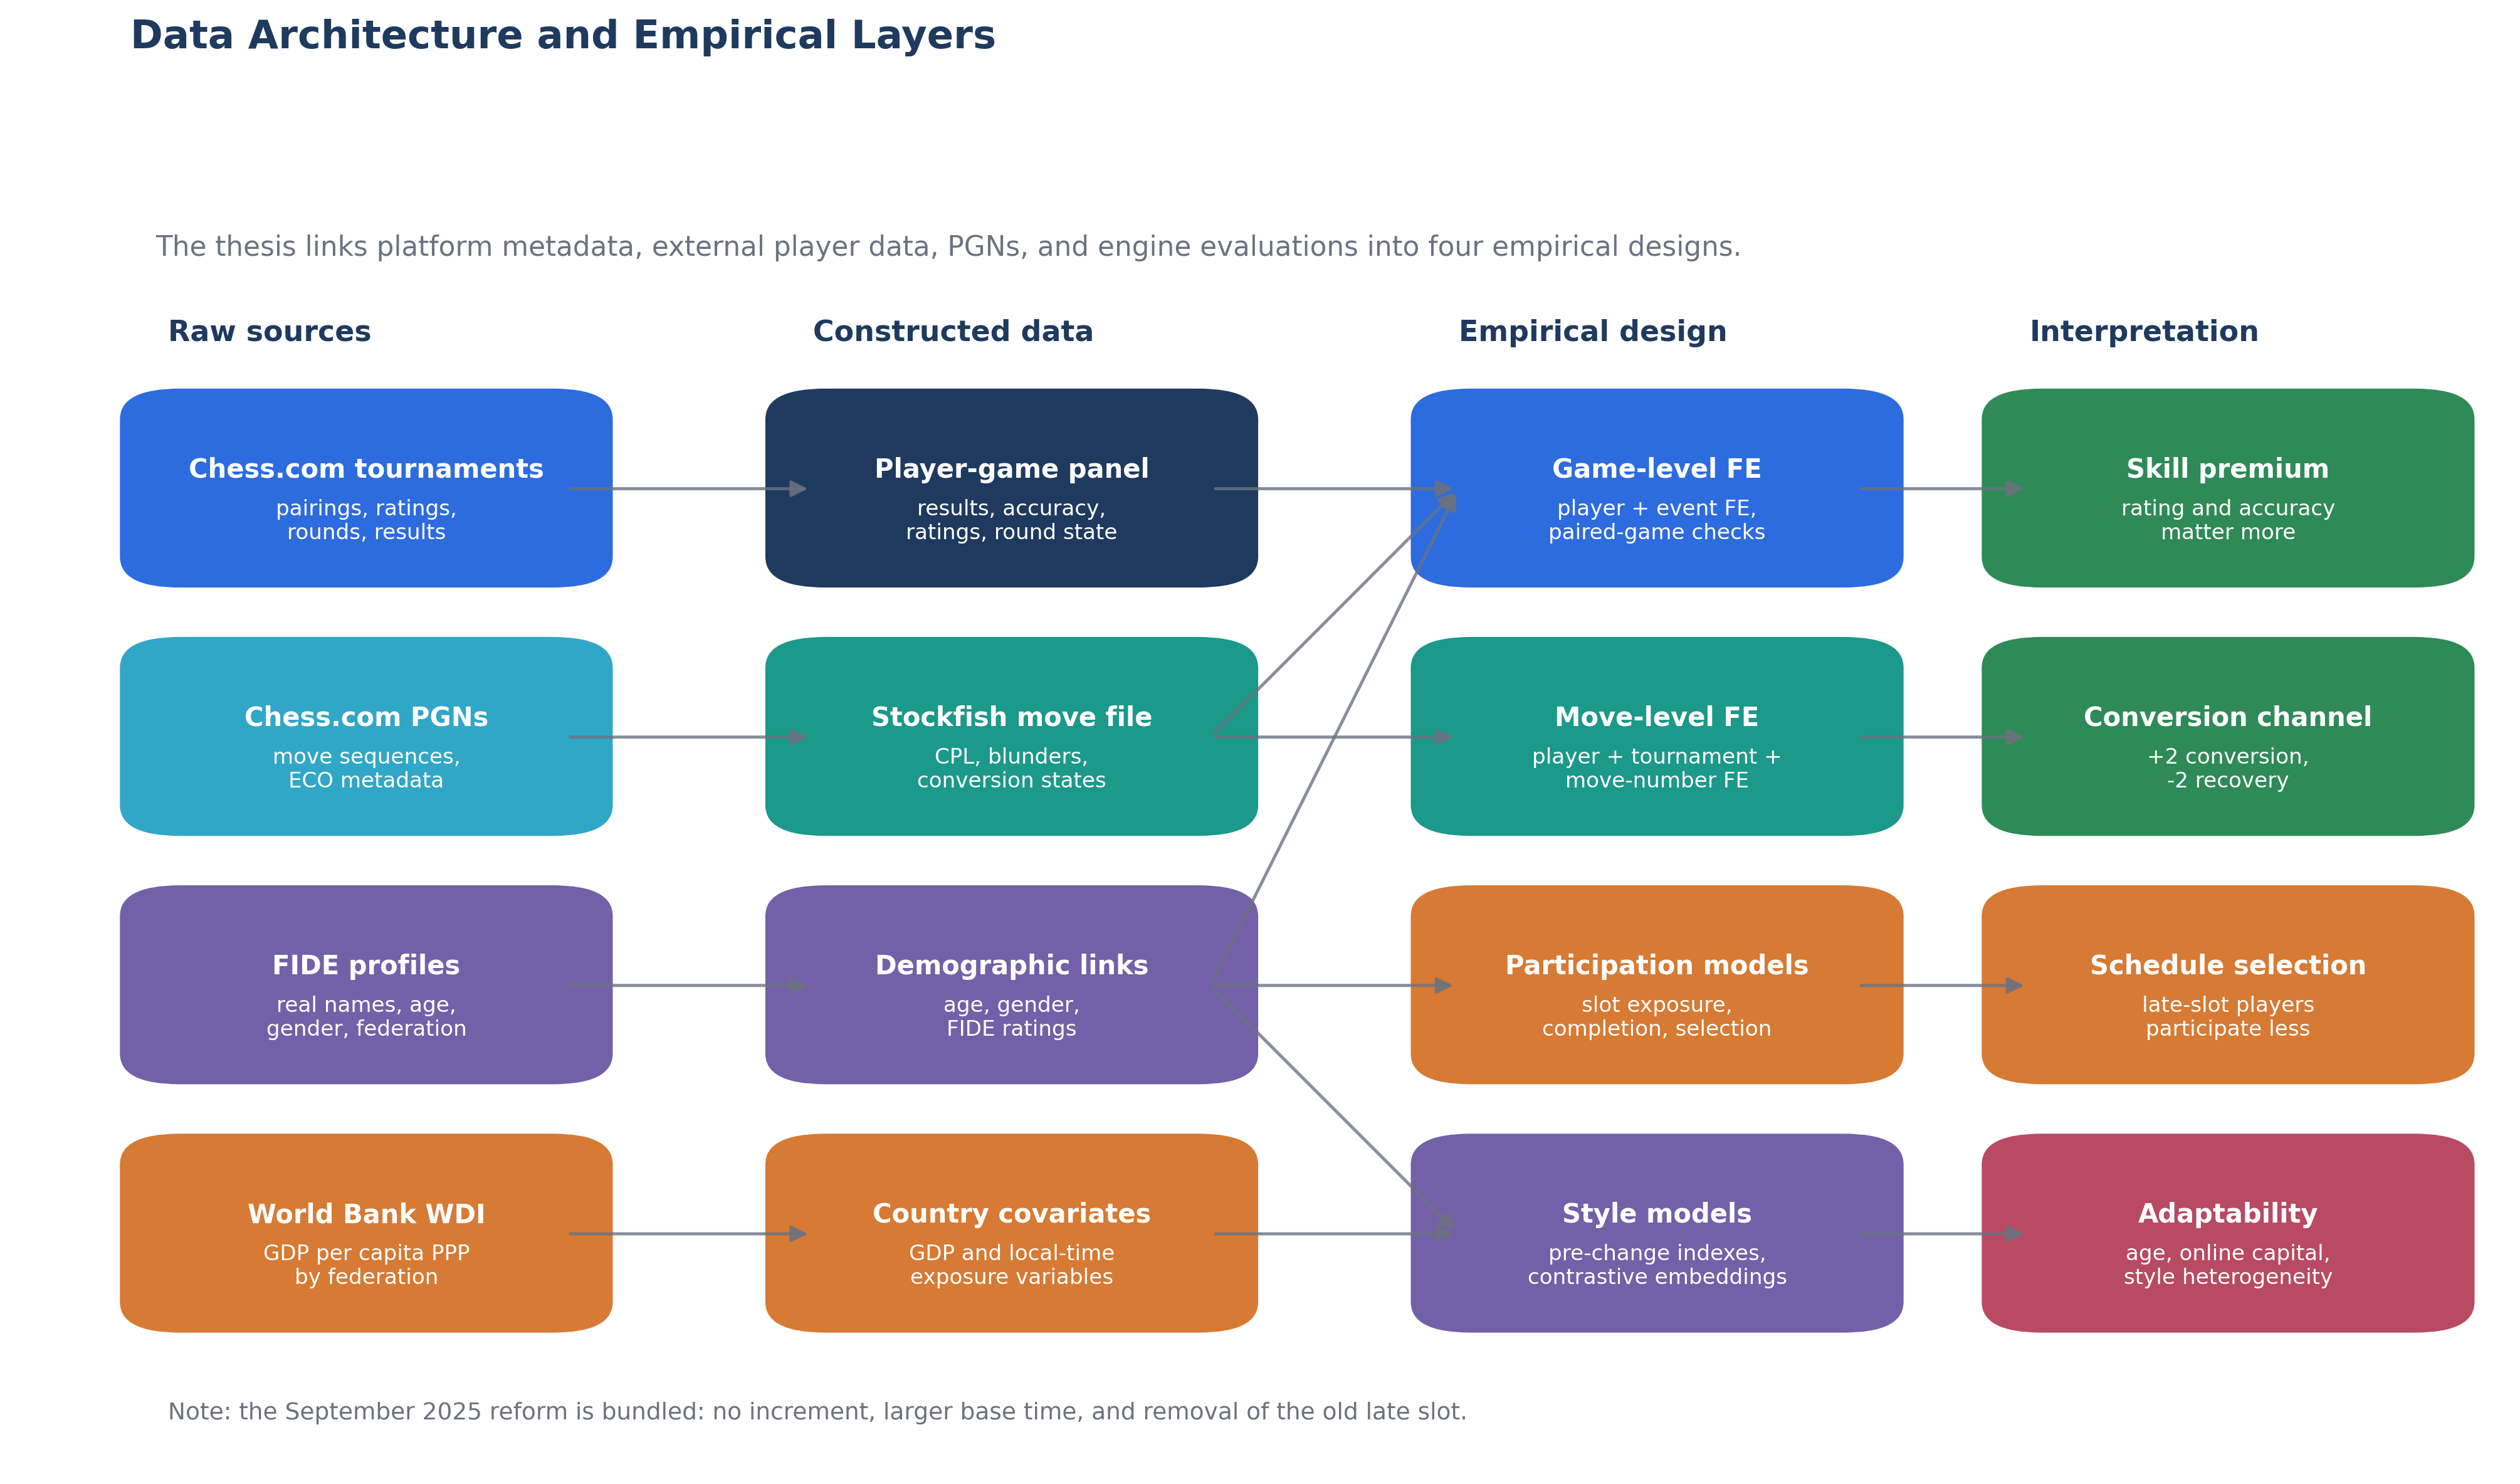
\includegraphics[width=\textwidth]{figures/figure7_data_design_map.png}
\caption{Data architecture and empirical layers used in the thesis.}
\label{fig:data-design-map}
\end{figure}

\subsection{Accuracy Variable Creation}

This variable is one of the key factors in our analysis. Chess.com accuracy is a game-level move-quality metric on a 0 to 100 scale. It is not identical to centipawn loss and Chess.com does not fully publish the exact proprietary formula, but it is widely understood by players and is available directly on many analyzed games. It is useful for the player-game production-function analysis because it provides a high-level measure of how well each player played in the game.

The main difficulty is missing data. Chess.com accuracy is available only after a game has been analyzed on Chess.com platform by someone. Strong or famous players are more likely to have games analyzed by viewers, stream audiences, or the players themselves. This creates a potential selection bias if analyzed games are systematically different from non-analyzed games. To reduce this problem, the project used an automated browser workflow to open game pages, trigger Chess.com's accuracy calculation where needed, wait for the analysis to complete, and then scrape the resulting accuracy. Because Chess.com pages are protected by anti-bot and Cloudflare systems, the collection process required robust browser automation, proxies, and CAPTCHA handling. The final accuracy dataset is therefore much closer to tournament coverage than the initially available analyzed-game subset.

Table \ref{tab:accuracy-summary} reports simple descriptive statistics for the accuracy variables in the main game metadata. White's mean accuracy is slightly higher than Black's, but the difference is small relative to the within-player and within-game variation used in the regressions.

\begin{table}[H]
\centering
\caption{Accuracy Summary by Color}
\label{tab:accuracy-summary}
\begin{tabular}{lrrrrr}
\toprule
Variable & Mean & Std. dev. & Min & Median & Max \\
\midrule
Accuracy White & 83.62 & 7.55 & 0.00 & 84.00 & 100.00 \\
Accuracy Black & 82.86 & 7.83 & 0.00 & 83.20 & 100.00 \\
\bottomrule
\end{tabular}
\end{table}

Table \ref{tab:metadata-summary} summarizes the main raw game-level variables before the most restrictive regression filters. Mean Chess.com ratings are around 2570 for both colors, which confirms that the sample consists of elite titled players. The mean White result is slightly above 0.5, consistent with the usual first-move advantage in chess. The analysis below does not rely on raw color comparisons because the main regressions control for color and include player and event fixed effects.

\begin{table}[H]
\centering
\caption{Selected Descriptive Statistics}
\label{tab:metadata-summary}
\begin{adjustbox}{max width=\textwidth}
\begin{tabular}{lrrrrrr}
\toprule
Variable & Mean & Std. dev. & Std. error & Min & Median & Max \\
\midrule
Rating White & 2576.49 & 285.67 & 0.42 & 0 & 2573 & 3319 \\
Rating Black & 2572.43 & 286.79 & 0.42 & 0 & 2568 & 3319 \\
Result White & 0.53 & 0.48 & 0.00 & 0 & 0.50 & 1 \\
Result Black & 0.47 & 0.48 & 0.00 & 0 & 0.50 & 1 \\
Accuracy White & 83.62 & 7.55 & 0.01 & 0 & 84.00 & 100 \\
Accuracy Black & 82.86 & 7.83 & 0.01 & 0 & 83.20 & 100 \\
\bottomrule
\end{tabular}
\end{adjustbox}
\end{table}

\subsection{Data Cleaning Rules}

Several cleaning rules are applied before the data science analysis. First, games with missing core identifiers, missing player names, missing event identifiers, or invalid results are removed (there are only $\approx100$ of them due to random access problems). Second, the analysis excludes observations from banned or anonymous accounts when these accounts cannot be linked to stable player identities. Third, games involving non-titled or improperly identified accounts are removed from specifications that require the titled-player population. Fourth, observations with impossible or placeholder ratings are dropped in specifications where rating differences are the key treatment interaction. Fifth, FIDE-based demographic and country variables are used only when the username-to-real-name match is sufficiently reliable. Ambiguous or unmatched cases are left missing for those specifications rather than forced into noisy demographic cells.

Accuracy-based models use additional restrictions. Games with accuracy equal to exactly 0 or exactly 100 are excluded from the main accuracy regressions. These values are often generated by missing analysis, parsing failures, very short games, or edge cases in Chess.com's accuracy display. Keeping them would mechanically create extreme values that are not comparable to normal analyzed games. The main accuracy models also exclude round 1 in some specifications, because first-round Swiss pairings can be unusually uneven and may mix the rule-change effect with mechanical pairing differences.

Move-level data require another layer of cleaning. PGNs must be parsable, moves must be legal from the reconstructed board state, and Stockfish evaluations must be available from the relevant player's perspective. Mate scores and extreme engine evaluations can produce very large centipawn losses. The main move-level regressions therefore use capped centipawn loss, \texttt{cp\_loss\_cap}, capped at 1000 centipawns. This preserves information about large mistakes while preventing a small number of mate-score positions from dominating linear models.

\subsection{PGN and Stockfish Data}

The move-level analysis uses PGNs scraped from Chess.com game links. The PGNs provide the sequence of moves, player names, game result, event information, opening metadata where available, clock annotations, and board states that can be reconstructed using a chess parser. For each move with a clock annotation, the pipeline records the player's clock after the move. The clock before the move is recovered from the previous own clock state, taking the time-control increment into account for 3+1 games. The difference gives \texttt{time\_spent}. The resulting variables include \texttt{time\_before\_move}, \texttt{time\_after\_move}, \texttt{time\_spent}, low-clock indicators at 5, 10, and 30 seconds, first entry into low-clock states, final clock, and clock reserves at moves 10, 20, and 30.

Stockfish was used to evaluate positions and moves. For each legal move in a parsed game, the script reconstructs the pre-move board, evaluates the position before and after the move from the mover's perspective, and computes centipawn loss. A move with a large loss relative to the engine benchmark is classified as an inaccuracy, mistake, or blunder using transparent thresholds: 50, 100, and 200 centipawns. The engine analysis was run in two scraping waves because the Chess.com PGN collection was built over time. 

The combined Stockfish mechanism sample used in the current thesis contains 70,868,483 centipawn rows read, 27,517,197 usable move rows after joining to metadata and applying filters, 319,095 games, 616,731 player-games, 5,768 players, and 148 tournaments. The broader clock-feature panel, which is used for the clock-specific mechanism tests, contains 1,556,230 matched player-games, 794,684 games, 7,947 players, 406 event time slots, and about 69.0 million weighted move observations. The gap between rows read and usable rows mostly comes from metadata matching and the fact that not all scraped PGN games are in the cleaned regression metadata.

\subsection{Variables Created on Move-Level}

The move-level variables capture both board-state mechanisms and clock-state mechanisms. Game phase is measured by fullmove number: opening moves 1--10, early middlegame moves 11--20, late middlegame moves 21--35, and endgame moves 36 and later. The variable \texttt{last\_10\_ply} marks the final ten individual moves of the game. These variables describe where in the game errors occur, while the recovered clock variables directly measure remaining-time states.

Critical positions are measured using engine evaluation. The main proxy, called critical equal in the code, equals one when the absolute pre-move engine evaluation from the mover's perspective is below 100 centipawns. This captures positions close to equality, where one mistake can shift the game. Conversion variables are defined at the player-game level. A player reaches a winning position if the engine evaluation reaches at least +200 centipawns from that player's perspective at least ten plies before the game ends. Conversion equals one if the player eventually wins. Similarly, a player reaches a losing position if the evaluation falls below -200 centipawns, and defensive escape equals one if the player eventually draws or wins.

Clock variables are constructed at both move and player-game levels. At the move level, the analysis uses clock bins \((>120, 60\text{--}120, 30\text{--}60, 10\text{--}30, 5\text{--}10, 0\text{--}5\) seconds), time spent on the move, whether the player starts or ends the move below 5, 10, or 30 seconds, and event-time indicators around the first crossing below a low-clock threshold. At the player-game level, the analysis aggregates these measures into low-clock exposure shares, mean time spent, final clock, move-10 clock reserve, low-clock centipawn loss, low-clock blunder rates, conversion while personally low on time, and conversion or escape when the opponent is low on time.

Additional PGN-derived features measure opening, complexity, simplification, and style. Opening depth is parsed from Chess.com's ECO and opening URL information. Complexity measures include legal-move counts, high-legal-move shares, pieces remaining, material remaining, and engine-evaluation volatility. Simplification variables include captures by move 20, queen-off indicators by moves 20 and 30, pieces remaining by move 30, material remaining by move 30, and a simplified-position indicator. These variables are mainly used to test mechanisms that later turn out to be weak or null.

\subsection{Style Features and Neural Data}

The style analysis uses only pre-change games to avoid post-treatment bias. Interpretable player-level style features are constructed from moves and Stockfish evaluations. The main indexes are:

\begin{itemize}
    \item \texttt{clean\_style\_index}: high no-blunder-game rate and low own error rates;
    \item \texttt{chaos\_creator\_index}: high eval-swing, captures, checks, decisive games, and opponent errors after the player's moves;
    \item \texttt{self\_risk\_index}: high own blunders, own mistakes, high upper-tail centipawn loss, and volatile own move quality;
    \item \texttt{practical\_chaos\_index}: chaos creation net of self-risk.
\end{itemize}

All component variables are winsorized at the 1st and 99th percentiles, standardized across players, averaged within each index, and then standardized again. The key advantage of this design is that style variables are predetermined relative to the reform.

For the neural style analysis, the same pre-change move data are converted into player-game move sequences after removing opening theory and the final moves of long games. The model specification, cluster construction, and cluster results are described together with the style findings in Section \ref{sec:playing-style}.
